
%(BEGIN_QUESTION)
% Copyright 2011, Tony R. Kuphaldt, released under the Creative Commons Attribution License (v 1.0)
% This means you may do almost anything with this work of mine, so long as you give me proper credit

A {\it steam eductor} is a device used to create a vacuum, by passing steam through a ``venturi'' tube.  In this process, a steam eductor is used to apply a constant venting suction to an oily water sump (underground storage vessel for collecting liquid):

$$\includegraphics[width=15.5cm]{i0005rx01.eps}$$

Calculate the amount of force applied to the ``manway'' cover on the sump when the educator is operating at its rated capacity, and also the direction of this force.

\vskip 10pt

Will the applied vacuum from the eductor help or hinder the two pumps' ability to move liquid out of the sump and to water treatment?  Will the effect be minimal or substantial?

\underbar{file i03465}
%(END_QUESTION)





%(BEGIN_ANSWER)

$F$ = 51.07 pounds of force, downward (holding the cover onto the flange).

\vskip 10pt

Although the eductor's suction will in fact hinder the pumps' ability to move liquid out of the sump to treatment, the effect will be minimal since 2 inches WC is tiny compared to the rated head (pressure) of the pumps at 40 feet WC.

%(END_ANSWER)





%(BEGIN_NOTES)

\vskip 20pt \vbox{\hrule \hbox{\strut \vrule{} {\bf Virtual Troubleshooting} \vrule} \hrule}

This question is a good candidate for a ``Virtual Troubleshooting'' exercise.  Presenting the diagram to students, you first imagine in your own mind a particular fault in the system.  Then, you present one or more symptoms of that fault (something noticeable by an operator or other user of the system).  Students then propose various diagnostic tests to perform on this system to identify the nature and location of the fault, as though they were technicians trying to troubleshoot the problem.  Your job is to tell them what the result(s) would be for each of the proposed diagnostic tests, documenting those results where all the students can see.

During and after the exercise, it is good to ask students follow-up questions such as:

\begin{itemize}
\item{} What does the result of the last diagnostic test tell you about the fault?
\item{} Suppose the results of the last diagnostic test were different.  What then would that result tell you about the fault?
\item{} Is the last diagnostic test the best one we could do?
\item{} What would be the ideal order of tests, to diagnose the problem in as few steps as possible?
\end{itemize}

%INDEX% Physics, fluids: pressure, force, and area
%INDEX% Process: oily water sump (realistic P&ID shown)

%(END_NOTES)

